% Report.
%
% Copyright (C) 2010  Vladimir Rutsky <altsysrq@gmail.com>
%
% This work is licensed under a Creative Commons Attribution-ShareAlike 3.0 
% Unported License. See <http://creativecommons.org/licenses/by-sa/3.0/> 
% for details.

% TODO: Use styles according to GOST (it's hard).

\documentclass[a4paper,10pt]{article}

% Encoding support.
\usepackage{ucs}
\usepackage[utf8x]{inputenc}
\usepackage[T2A]{fontenc}
\usepackage[russian]{babel}

\usepackage{amsmath, amsthm, amssymb}

% Indenting first paragraph.
\usepackage{indentfirst}

\usepackage{url}
\usepackage[unicode]{hyperref}

%\usepackage[final]{pdfpages}

\usepackage[pdftex]{graphicx}
\usepackage{subfig}

%TODO: use texments
\usepackage{listings}

\newcommand{\HRule}{\rule{\linewidth}{0.5mm}}

% Spaces after commas.
\frenchspacing
% Minimal carrying number of characters,
\righthyphenmin=2

% From K.V.Voroncov Latex in samples, 2005.
\textheight=24cm   % text height
\textwidth=16cm    % text width.
\oddsidemargin=0pt % left side indention
\topmargin=-1.5cm  % top side indention.
\parindent=24pt    % paragraph indent
\parskip=0pt       % distance between paragraphs.
\tolerance=2000
%\flushbottom       % page height aligning
%\hoffset=0cm
%\pagestyle{empty}  % without numeration

\newcommand{\myemail}[1]{%
\href{mailto:#1}{\nolinkurl{#1}}}

\begin{document}

% Title page.
% title.tex
% Report title page.
% Copyright (C) 2010  Vladimir Rutsky <altsysrq@gmail.com>

\begin{titlepage} % начало титульной страницы

\begin{center} % включить выравнивание по центру

\large Санкт-Петербургский государственный политехнический университет\\[5.5cm]
% название института, затем отступ 5,5см

\huge Отчет по курсовой работе\\[0.6cm] % название работы, затем отступ 0,6см
\large по~курсу <<Верификация программ>>\\[1cm]
\large <<Разработка контроллера светофоров на перекрёстке и его верификация>>\\[6cm]
% тема работы, затем отступ 6см

\begin{flushright} % выровнять её содержимое по правому краю
\begin{tabular}{l l}
Студент: & Руцкий~В.\,В.\\
Группа: & 5057/2\\
Вариант: & 9, 13\\
Преподаватель: & Шошмина~И.\,В.
\end{tabular}
\end{flushright} % конец выравнивания по правому краю

\vfill % заполнить всё доступное ниже пространство

{\large Санкт-Петербург 2010}
\end{center} % закончить выравнивание по центру
\thispagestyle{empty} % не нумеровать страницу
\end{titlepage} % конец титульной страницы


\tableofcontents
\pagebreak

% Content

\section{Постановка задачи}
Задан автомобильный перекрёсток, его конфигурация показана на рис.~\ref{fig:crossroad} (вариант 9, 13).
\begin{figure}[h!]
  \centering
  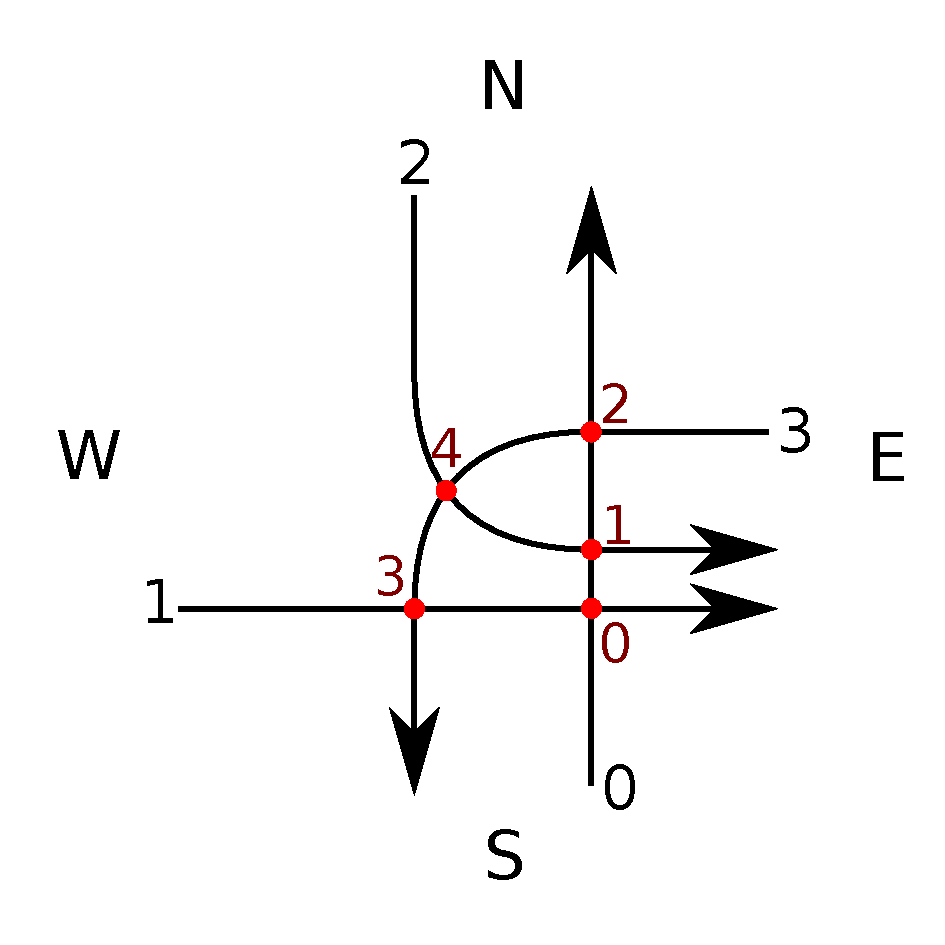
\includegraphics[width=0.5\linewidth]{./data/crossroad.pdf}
  \caption{Схема перекрёстка}
  \label{fig:crossroad}
\end{figure}
На перекрёстке возможны следующие направления движения транспорта:
\begin{itemize}
  \item $\mathrm{S} \rightarrow \mathrm{N}$,
  \item $\mathrm{W} \rightarrow \mathrm{E}$,
  \item $\mathrm{N} \rightarrow \mathrm{E}$,
  \item $\mathrm{E} \rightarrow \mathrm{S}$,
\end{itemize}
Каждое направление движения регулируется собственным светофором.
На каждом направлении движения установлены датчики, фиксирующие наличие автомобилей.

При отсутствии автомобилей на полосе, соответствующий светофор должен гореть красным светом.
При появлении машин на полосе, соответствующий светофор должен убедиться, 
что по всем пересекающимся с текущей полосам движение транспорта запрещено 
(их светофоры горят красным), и загореться зелёным светом.
При наличии машин на различных полосах, светофоры должны периодически переключаться, 
обеспечивая равномерный пропуск машин по всем направлениям.

Требуется разработать модель управления данным светофором на языке \textit{Promela}, 
удовлетворящую указанным выше требованиям, 
и верифицировать её корректность с помощью пакета \textit{Spin}%
\footnote{\url{http://www.spinroot.com/}}.

\section{Решение}



\subsection{Верификация алгоритма}


\subsection{Проверка корректности}

\section{Результат работы}
В результате работы ...

\appendix
\section{Исходный код}

\lstinputlisting[language=c]{data/main.pml}

\bibliographystyle{unsrt}
\bibliography{references.bib}

\end{document}
